%%%%%%%%%%%%%%%%%%%%%%%%%%%%%%%%%%%%%%%%%
% Beamer Presentation
% Ricks Template
%
%
%%%%%%%%%%%%%%%%%%%%%%%%%%%%%%%%%%%%%%%%%

%----------------------------------------------------------------------------------------
%	PACKAGES AND THEMES
%----------------------------------------------------------------------------------------
\documentclass[t,aspectratio=169,11pt,presentation]{beamer}
%\documentclass[t,aspectratio=169,11pt,presentation]{beamer}
%\documentclass[t,aspectratio=169,11pt,draft]{beamer}


% Define colors
\definecolor{ptb5}{RGB}{54,75,154}	 % NT                   
\definecolor{ptb4}{RGB}{74,123,183} % RC + NT	                    
\definecolor{ptb3}{RGB}{110,166,205}                     
\definecolor{ptb2}{RGB}{152,202,225}% EC + RC + NT                  
\definecolor{ptb1}{RGB}{194,228,239}
\definecolor{ptg0}{RGB}{234,236,204}
\definecolor{ptr1}{RGB}{254,218,139} %EC only
\definecolor{ptr2}{RGB}{253,179,102}	                    
\definecolor{ptr3}{RGB}{246,126,75} % AT +	EC + RC                    
\definecolor{ptr4}{RGB}{221,61,45}	 % AT + EC                   
\definecolor{ptr5}{RGB}{165,0,38}	 % AT	   

\usetheme{Boadilla}




% Footer and page numbers

% First remove the navigation symbols from the bottom of all slides 
\setbeamertemplate{navigation symbols}{} 

% Remove the colored line at the bottom
\setbeamertemplate{footline}{}


% Customize items
\setbeamertemplate{itemize items}{\color{ptb2}{\rule[0.05em]{0.6em}{0.6em}}}
\setbeamertemplate{itemize subitem}{\color{ptb2}{\raisebox{0.12em}{$\blacktriangleright$}}}
\setbeamercolor{enumerate item}{fg=black}
\setbeamertemplate{enumerate item}[default]
\setbeamercolor{enumerate subitem}{fg=black}
\setbeamertemplate{enumerate subitem}[default]


\setbeamercolor{subsection in toc}{bg=white,fg=black}




% Table of Contents (if we have one)
\setbeamertemplate{section in toc}{\inserttocsectionnumber.~\inserttocsection}
\setbeamercolor{section in toc}{bg=white,fg=black}
\setbeamertemplate{subsection in toc}{%
  \hspace{1.2em}{{\color{ptb5}{\rule[0.05em]{0.6em}{0.6em}}}~\inserttocsubsection\par}
}
\setbeamercolor{subsection in toc}{bg=white,fg=black}


% Customize beamer colors

\setbeamercolor{titlelike}{fg=white,bg=ptb5}
\setbeamercolor{button}{bg=ptb4,fg=white}
%}

% Nicer looking Itemize and enumerate environments
\newenvironment{wideitemize}{\itemize\addtolength{\itemsep}{14pt}}{\enditemize}
\newenvironment{wideenumerate}{\enumerate\addtolength{\itemsep}{14pt}}{\endenumerate}

% Import packages
\usepackage[default]{lato} % More modern looking font than Helvetica
\usepackage{geometry,caption,color,setspace,dsfont,commath,amsmath,amssymb,bm,mathrsfs}
\usepackage[normalem]{ulem}
\usepackage[comma]{natbib}
\usepackage[short]{optidef}
\usepackage{hhline}
\usepackage{array}
\usepackage{booktabs} % Allows the use of \toprule, \midrule and \bottomrule in tables
\usepackage{adjustbox}
\usepackage{graphicx,xcolor,bbm,xcomment}
\usepackage{appendixnumberbeamer}
\usepackage{textcomp}
\usepackage{colortbl}
\usepackage{subcaption} 
\usepackage{tikz}
\usetikzlibrary{calc,patterns,positioning}
\usepackage{pdflscape}
\usepackage{environ}
\usepackage{array}
\usepackage{etoolbox}
\usepackage[normalem]{ulem}
\BeforeBeginEnvironment{itemize}{\par}
\BeforeBeginEnvironment{enumerate}{\par}

\bibliographystyle{ecta}

\newcommand*\diff{\mathop{}\!\mathrm{d}}


% Make Section Header Frames
\AtBeginSection[]{

  \setbeamercolor{titlelike}{bg=ptb5,fg=white}
  \setbeamertemplate{navigation symbols}{} 
  \begin{frame}[noframenumbering]
  \vfill
  \centering
  \begin{beamercolorbox}[sep=8pt,center,shadow=true,rounded=true]{title}
    \usebeamerfont{title}\insertsectionhead\par%
  \end{beamercolorbox}
  \vfill
  \end{frame}
  % Make a new prettier page number
\addtobeamertemplate{navigation symbols}{}{%
    \usebeamerfont{footline}%
    \hspace{5em}%
    {\color{black!50}{\small\insertframenumber/\inserttotalframenumber}}%
}
\setbeamercolor{titlelike}{fg=ptb5,bg=white}
}

\AtBeginSubsection[]{
  \setbeamertemplate{navigation symbols}{} 
  \begin{frame}[noframenumbering]
  \vfill
  \centering
  \begin{beamercolorbox}[sep=8pt,center,shadow=false,rounded=true]{title}
    \usebeamerfont{title} \insertsubsectionhead\par%
  \end{beamercolorbox}
  \vfill
  \end{frame}
  % Make a new prettier page number
\addtobeamertemplate{navigation symbols}{}{%
    \usebeamerfont{footline}%
    \hspace{5em}%
    {\color{black!50}{\small\insertframenumber/\inserttotalframenumber}}%
}
}



\tikzset{
    invisible/.style={opacity=0},
    visible on/.style={alt={#1{}{invisible}}},
    alt/.code args={<#1>#2#3}{%
      \alt<#1>{\pgfkeysalso{#2}}{\pgfkeysalso{#3}} % \pgfkeysalso doesn't change the path
    },
  }
  
  
\makeatletter
\newsavebox{\measure@tikzpicture}
\NewEnviron{scaletikzpicturetowidth}[1]{%
  \def\tikz@width{#1}%
  \def\tikzscale{1}\begin{lrbox}{\measure@tikzpicture}%
  \BODY
  \end{lrbox}%
  \pgfmathparse{#1/\wd\measure@tikzpicture}%
  \edef\tikzscale{\pgfmathresult}%
  \BODY
}
\makeatother

\tikzset{
  pics/student/.style args={#1,#2}{
     code={
       \filldraw [fill=#1,draw=black,visible on=#2] (.05,.15) .. controls (.05,.7) and (.65,.8) .. (.75,.2) .. controls (.55,.05) and (.05,0) .. (.05,.15) ;
       \filldraw [fill=#1,draw=black,visible on=#2] (.35,.75) circle [radius=.22];
     }
  }
}

%----------------------------------------------------------------------------------------
%	TITLE PAGE
%----------------------------------------------------------------------------------------
 

\title{From Value Added to Welfare Added: \\ A Social Planner Approach to Education Policy and Statistics\vskip.3cm}

\author{Tanner S Eastmond\footnote{Department of Economics, University of California San Diego} \vskip.2cm Nathan Mather$^2$ \vskip.2cm Michael Ricks\footnote{Department of Economics, University of Michigan} \vskip.2cm Julian Betts\footnote{Department of Economics, University of California San Diego and NBER} }

\begin{document}

\begin{frame}[noframenumbering]
\maketitle
\end{frame}


\setbeamercolor{titlelike}{fg=ptb5,bg=white}
% Make a new prettier page number
\addtobeamertemplate{navigation symbols}{}{%
    \usebeamerfont{footline}%
    \hspace{5em}%
    {\color{black!50}{\small\insertframenumber/\inserttotalframenumber}}%
}



%------------------------------------------------

% Why do we care about late entry
%------------------------------------------------
\begin{frame}{\textbf{ } }

\begin{wideitemize}
    \item 
    
    \item <2->
    \begin{itemize}
        \item<3-> 
        \item<4-> 
    \end{itemize}
    
    \item<5-> {\color<5>{ptr5}\textbf{Question1}} 
  
    \item<6> {\color<6>{ptr5}\textbf{Question2}}
  
\end{wideitemize}

\end{frame}

%------------------------------------------------
\begin{frame}{\textbf{ } }

\begin{wideitemize}
    \item 
    
    \item <2->
    \begin{itemize}
        \item<3->{\color<3>{ptr5}\textbf{Impacts}}: If policies have distinct affects on different groups  
        \item<4->{\color<4>{ptr5}\textbf{Outcomes}}: If policies affect multiple outcomes in different ways
        \item<5->{\color<5>{ptr5}\textbf{Preferences}}: If policymakers assign varried value to different groups (e.g., care about levels \textbf{and} gaps)
    \end{itemize}
    
    \item<5-> (NCLB)
  
    \item<6> 
  
\end{wideitemize}

\end{frame}
%------------------------------------------------



%------------------------------------------------
% What do we know about late entry effects
\begin{frame}{\textbf{}}

\begin{wideitemize}
    \item We need to know how waiting affects children who {\color{ptb4}\textbf{reluctantly}} and {\color{ptr5}\textbf{always}} wait
    
    \item<2-> \textbf{Causal research}: Compare children around birthday cutoffs to measure gains
    
    \begin{itemize}
        %\item Compare children with birthdays just before and after state cutoffs
        \item Older ``entry age'' increases achievement, advanced course taking, and college persistence
        
         {\tiny \color{gray}\citep[e.g.,][etc.]{datar2006does,deming2008lengthening,elder2009kindergarten,dhuey2019school,routon2020older}}
        
        \item<3-> IVs identify Local Average Treatment Effects (LATE) of {\color{ptr2}\textbf{eager}} recommendation following
        % The compliers are...
        
        % They are different observably
        % They are making different decisions
    \end{itemize}
    
    \item<4-> \textbf{Descriptive research}: Compare children whose parents made different decisions
    

    \begin{itemize}
        \item Families who don't follow recommendations are systematically different
        % This could mean that there is efficient sorting, but it might not. two narratives about equity suggest that
        
        {\tiny \color{gray} \citep[e.g.,][]{cameron1990effects,graue2000redshirting,march2005academic,schanzenbach2017your,fortner2017kindergarten}}
    
        \item<5-> There is no reason that the LATE would be externally valid
    \end{itemize}
    
    \item<6-> \textbf{This paper}: Estimate effects on {\color{ptb4}\textbf{reluctant}}, {\color{ptr2}\textbf{eager}}, and  {\color{ptr5}\textbf{always}} waiting children
    
    %cannot inform counterfactual policy discussions about reducing noncompliance or economic questions about efficiency and equity. This is because these questions hinge on the sorting of and effects on noncompliant children---patterns the complier-based LATE cannot inform.
    

\end{wideitemize}
\end{frame}

% Maybe show a figure of the RD in my data?

%------------------------------------------------
% What is my question and how will I answer it?
\begin{frame}{\textbf{This paper will estimate effects of waiting on each group}}

\begin{wideitemize}
    \item I answer these questions using data on the universe of kindergarteners in Michigan
    \begin{itemize}
        \item Focus on one cohort of children facing a cutoff in 2013 
        \item Measure academic outcomes at third grade
    \end{itemize}
    
    
    \item<2-> Two birthday cutoffs $\to$ effects on children who {\color{ptr2}\textbf{eagerly}} and {\color{ptb4}\textbf{reluctantly}} wait
    
    \begin{itemize}
        \item {\color<3-4>{ptr2}\textbf{First cutoff}}: recommends waiting
        \item {\color<5-6>{ptb4}\textbf{Second cutoff}}: requires waiting
        
        
        {\tiny \color{gray} \citep{cattaneo2016interpreting,cattaneo2020extrapolating}}
    
    \end{itemize}    
    \end{wideitemize}
\only<2-6>{
    \vspace{1em}
    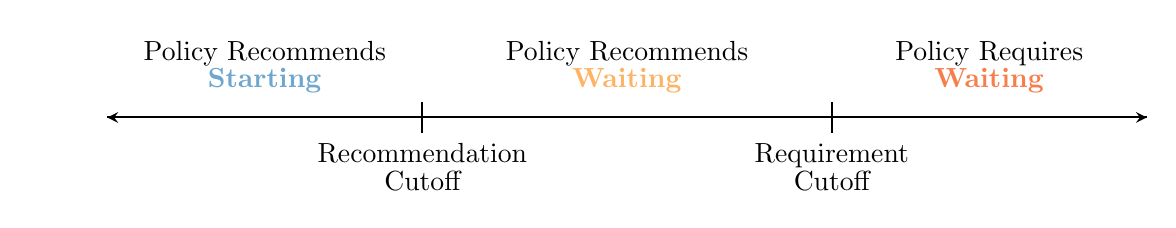
\begin{tikzpicture}
    \draw [font=\fontsize{10pt}{10pt}\selectfont,outer sep = 4pt,line width=.025cm,visible on=<2->] (-6.6,-1.2)  -- node [anchor=south,align=center,minimum height = 1cm,visible on=<3->] {Policy Recommends \\ {\color{ptb3}\textbf{Starting}}} (-2.6,-1.2);
    \draw [font=\fontsize{10pt}{10pt}\selectfont,outer sep = 4pt,line width=.025cm,visible on=<2->] (-2.6,-1.2) -- node [anchor=south,align=center,minimum height = 1cm,visible on=<4->] {Policy Recommends \\ {\color{ptr2}\textbf{Waiting}}} (2.6,-1.2);
    \draw [font=\fontsize{10pt}{10pt}\selectfont,outer sep = 4pt,line width=.025cm,,visible on=<2->] (2.6,-1.2) -- node [anchor=south,align=center,minimum height = 1cm,visible on=<6->] {Policy Requires \\ {\color{ptr3}\textbf{Waiting}}} (6.6,-1.2);
    
    \draw [font=\fontsize{10pt}{10pt}\selectfont,line width=.025cm,color=white,visible on=<2->] (-7.6,-1.2) -- (-6.6,-1.2) ;
    \draw [font=\fontsize{10pt}{10pt}\selectfont,line width=.025cm,stealth-stealth,visible on=<2->] (-6.6,-1.2) -- (6.6,-1.2) ;
    \draw [font=\fontsize{10pt}{10pt}\selectfont,line width=.025cm,visible on=<2->] (-2.6,-1.4) node [anchor=north,align=center] {Recommendation \\ Cutoff} -- (-2.6,-1.) ;
    \draw [font=\fontsize{10pt}{10pt}\selectfont,line width=.025cm,visible on=<2->] (2.6,-1.4) node [anchor=north,align=center] {Requirement \\ Cutoff}-- (2.6,-1.) ;
    \end{tikzpicture}
        \vspace{-30em}}
    
\begin{wideitemize}
    
    \item<8-> No discontinuity affects children who {\color{ptr5}\textbf{always}} wait
    
    
     \begin{itemize}
         \item<9-> \textbf{New test}: Changes in test scores over birthdays identify selection
         \item<9-> Extrapolation using either regression discontinuity or marginal treatment effects tools
         
        {\tiny \color{gray} \citep{heckman2005structural,brinch2017beyond,mogstad2018using,cattaneo2020extrapolating}}
     
     \end{itemize}

\end{wideitemize}
\end{frame}

%------------------------------------------------
% What is the answer
\begin{frame}{\textbf{Parental selection increases achievement but reduces equity}}

            
\begin{wideitemize}
%\item There is significant selection:
% Recall I am thinking about selection in terms of potential untreated outcomes
\item {\color<1>{ptr5}\textbf{Negative selection in levels:}} Parents make lower achieving children wait 

{\tiny \color{gray}\citep{cameron1990effects,march2005academic,schanzenbach2017your,fortner2017kindergarten}}


\item<2-> {\color<2>{ptr5}\textbf{Positive selection on gains:}} Strategic entry raises average achievement

{\tiny \color{gray} \citep{bedard2006persistence,black2011too,mccrary2011effect,cook2016birthdays,molnar2018redshirting,fortner2019forced}}

\begin{itemize}
    \item<3-> {\color<3>{ptr5}\textbf{Differential Sorting:}} Response to gains is driven by higher-income families 
 
    {\tiny \color{gray} \citep[]{lalonde1986evaluating,brand2010benefits,einav2010optimal,walters2018demand,finkelstein2019take,ito2021selection}}
\end{itemize}

%brinch2017beyond,mogstad2018using,kline2019heckits,walters2018demand,ito2021selection


\item<4-> {\color<4>{ptr5}\textbf{Unequal Impacts:}} Strategic entry expands achievement gaps

{\tiny \color{gray} \citep[]{graue2000redshirting,deming2008lengthening,illinois2019anact}}


\begin{itemize}
    \item<5-> {\color<5>{ptr5}\textbf{Early Investments:}} Public investment could shrink gaps and raise scores

    {\tiny \color{gray} \citep{elder2009kindergarten,kline2016evaluating,felfe2018does,cornelissen2018benefits,shapiro2019if}}
    
\end{itemize}

    
   

% This is for two reasons...


%\begin{itemize}
%    \item<11-> Average gains are $0.48$ for high SES but only $0.16$ for low SES
%    \item<12-> Only high-income families sort children on gains
%\end{itemize}
\end{wideitemize}



%main implications for what we don't know:
%\begin{itemize}    
%    \item Parents redshirt child if (1) they can AND (2) they think their child needs it
%    \item Parents are making (short term) optimal decisions for their children
%    \item Parents' decisions have (short term) positive externalities for other children
  
\end{frame}





\setbeamertemplate{navigation symbols}{} 
  
%-----------------------------------------------
\begin{frame}[c,noframenumbering]{Today's Talk}

\begin{columns}
\begin{column}{0.575\textwidth}
\vspace{-1.5em}
\begin{wideenumerate}
    \item How Should We Model Decision-making?
    \begin{itemize}
        \item Kindergarten Entry
        \item Waiting and Achievement
        \item Equity and Efficiency
    \end{itemize}
    \item How Do Entry Decisions Affect Children?
    \begin{itemize}
        \item Michigan Policy and Data
        \item RD Estimates
        \item MTE Estimates
    \end{itemize}
    \item What About Welfare and Policy?
\end{wideenumerate}
\end{column}
\begin{column}{0.40\textwidth}
\vspace{-1.5em}

\begin{tikzpicture}
%\draw[line width=.5cm] (0,0)  -- (3.2,1.8) -- (0,3.5) -- (3,4.2);
\usetikzlibrary{arrows}
\usetikzlibrary{shapes}
\tikzstyle{every node}=[draw=black,fill=black, ellipse]
\node[minimum width=2.6cm, minimum height = 1cm] (a) at (0,0) {};
\node[minimum width=2cm, minimum height = .8cm] (b) at (4,1.6) {};
\node[minimum width=1.6cm, minimum height = .6cm] (c) at (0,3.2) {};
\node[minimum width=1.2cm, minimum height = .4cm] (d) at (3.2,3.9) {};
\draw[fill = black] (a.75) -- (b.188) -- (b.235) -- (a.06);
\draw[fill = black] (b.170) -- (c.318) -- (c.348) -- (b.140);
\draw[fill = black] (c.5) -- (d.205) -- (d.182) -- (c.28);
\draw[fill = black]  (2.8,5.5) to  [bend right=14] (3.2,4.6) to [bend right =14] (3.6,5.5) -- cycle;
\draw[fill = black] (3.6,5.5) arc (0:180:.4cm);
\draw[fill = white] (3.2,5.5) circle (.22cm);

\end{tikzpicture}



\end{column}
\end{columns}
\end{frame}


\addtobeamertemplate{navigation symbols}{}{%
    \usebeamerfont{footline}%
    \hspace{5em}%
    {\color{black!50}{\small\insertframenumber/\inserttotalframenumber}}%
}

%------------------------------------------------
\section{How Should We Think About Kindergarten Entry Decisions?}


	\begin{frame}[label=wait1]{\textbf{First stage: To wait or to start kindergarten } }
		
    
    \begin{figure}
        \centering
        \begin{scaletikzpicturetowidth}{\textwidth}
        \input{Slides/tables_figures/practice_talk/UD_unspool2}
        \end{scaletikzpicturetowidth}
    \end{figure}
		
		
	\vfill
	\hyperlink{model1}{\beamerbutton{Formal Model 1}}  
	\hyperlink{whywaiting}{\beamerbutton{Why ``Waiting''?}}  
	\hyperlink{treatments}{\beamerbutton{Definitions of Treatment}}  

		
		
	\end{frame}
	

	\begin{frame}{\textbf{Second stage: Waiting decisions and test scores}}
		\begin{wideitemize}
			
			\item Define potential third grade achievement if start/wait: $Y(w)=Y_w(X,r,U,\gamma_w)$
			
			\item<2-> Average potential outcomes by group$: g\in\{at, ec, rc\}$

			\[  \mu_{w,g}(r,x) = \mathbb{E}[Y_i(w)|R_i=r,G_i=g,X=x] \]
				
		\begin{center}
			\input{Slides/tables_figures/practice_talk/intro_framework2}
		\end{center}	
				
				
			\item<7-> {\color{ptr5}\textbf{Positive Question: How do families select into waiting? 	}}
				
			\hypertarget<7>{wait2}{}
				

		\end{wideitemize}
		

		
		
		\hyperlink{model2}{\beamerbutton{Formal Model 2}}
	\end{frame}
	
	
	
	
	\begin{frame}[label=wait3]{\textbf{Welfare: Selection, efficiency, and equity}}
		\begin{wideitemize}
			\item<2-> {\color<2-4>{ptr5}\textbf{Normative Question: Does allowing choice make families better off on average?}}
			\begin{itemize}
				% Efficient if not
				\item Efficiency $=$ choices are revealed preferred and result in higher average scores
				
				%{\tiny \color{gray} \citep[e.g.,]{carneiro2011estimating,kaufmann2014understanding,nybom2017distribution}}
				
				\item<3->This assumes \textbf{no spillovers in utility} among families
				%Noncompliance could reduce efficiency because the children who benefit the most are often least likely to participate.
				% This may be the rationale behind rules banning early entry in 15 states
				%\item<4-> Noncompliance might also be inefficient if positive selection drives achievement
				
				%{\tiny \color{gray} \citep[][]{schanzenbach2017your,fortner2017kindergarten}}
				
				% In any of these cases there is a social cost of having kids who benefit less wait to enter
				\item<4-> Certain spillovers in scores among families could also be an issue
				
				{\tiny \color{gray} \citep{bedard2012school,cascio2016first,pena2017creating}}
				
			\end{itemize}
			
			\item<5-> {\color<5>{ptr5}\textbf{Normative Question: Does strategic entry widen or shrink social disparities?}}
			\begin{itemize}
				\item Equitable $=$ choice does not widen differences across groups
				
				%\item<6>  White and higher-income families are more likely to exercise choice
				
				%{\tiny \color{gray} \citep[][]{schanzenbach2017your,fortner2017kindergarten}}
				
				
				%\item<6-> privileged families can sort more efficiently on gains
				%\item<7-> their children benefit more from waiting on average
			\end{itemize}
				
			\item<6> I can assess both sets implications of choice if I know $\mu$ by $x$
			
			
			% Concern about this inequity is strong enough that noncompliance is banned in many states and school districts.
			% Note the tension between equity and efficiency questions
		\end{wideitemize}
		\vspace{4em}
		%\hyperlink{equity}{\beamerbutton{Equity Algebra}}    
		\hyperlink{narratives}{\beamerbutton{Common Assumptions About Selection}}    
	\end{frame}




%------------------------------------------------
\section{How Does Waiting to Enter Kindergarten Affect Children?}
\subsection{Michigan Context: Policy and Data}

%------------------------------------------------
\begin{frame}{\textbf{Michigan policy context has extra identifying variation}}


\begin{wideitemize}
    \item Most states have birthday cutoffs that {\color<1>{ptb3}\textbf{recommend}} entry decisions %($z\in{0,1}$)
    %\begin{itemize}
    %    \item Nationwide we see 6-7\% always takers and at least 2-3\% reluctant compliers 
    %\end{itemize}
    %Redshirting has always been allowed, but some early entry has been essentially prohibited since 2010 (districts receive no state funding for enrolled children who have not turned five by December 1). 
    \item<2-> 15 states and many districts {\color<2>{ptr3}\textbf{require}} waiting after the cutoff  %($z\in{0,2}$)
      \begin{itemize}
        \item And many are considering requiring starting before the cutoff (as in many other countries)
        
        {\tiny \color{gray}\citep[e.g.][]{illinois2019anact}}
    \end{itemize}  
    \item<3-> Michigan has had both policies at {\color<3->{ptr5}\textbf{two}} sequential cutoffs \only<8-9>{(I focus on one cohort)} \hypertarget<9>{policy1}{}


\end{wideitemize}
  
    \vspace{2em}
    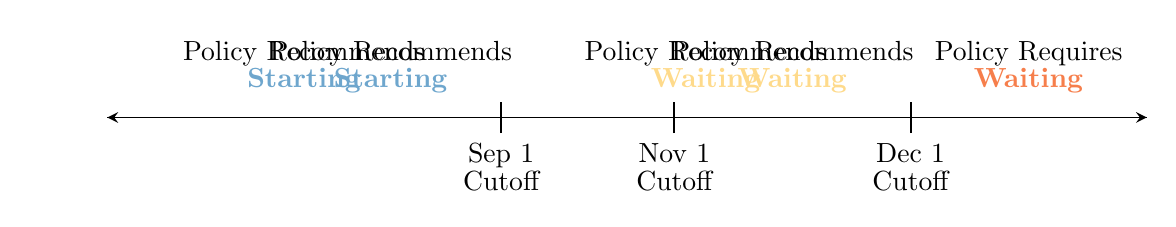
\begin{tikzpicture}
    \draw [font=\fontsize{10pt}{10pt}\selectfont,outer sep = 4pt,line width=.025cm,visible on=<4-8>] (-6.6,-1.2)  -- node [anchor=south,align=center,minimum height = 1cm,visible on=<5-8>] {Policy Recommends \\ {\color{ptb3}\textbf{Starting}}} (-1.6,-1.2);
    \draw [font=\fontsize{10pt}{10pt}\selectfont,outer sep = 4pt,line width=.025cm,visible on=<9->] (-6.6,-1.2)  -- node [anchor=south,align=center,minimum height = 1cm,visible on=<9->] {Policy Recommends \\ {\color{ptb3}\textbf{Starting}}} (0.6,-1.2);
    
    \draw [font=\fontsize{10pt}{10pt}\selectfont,outer sep = 4pt,line width=.025cm,visible on=<4-8>] (-1.6,-1.2) -- node [anchor=south,align=center,minimum height = 1cm,visible on=<6-8>] {Policy Recommends \\ {\color{ptr1}\textbf{Waiting}}} (3.6,-1.2);
    \draw [font=\fontsize{10pt}{10pt}\selectfont,outer sep = 4pt,line width=.025cm,visible on=<9->] (0.6,-1.2) -- node [anchor=south,align=center,minimum height = 1cm,visible on=<9->] {Policy Recommends \\ {\color{ptr1}\textbf{Waiting}}} (3.6,-1.2);
    \draw [font=\fontsize{10pt}{10pt}\selectfont,outer sep = 4pt,line width=.025cm,,visible on=<4->] (3.6,-1.2) -- node [anchor=south,align=center,minimum height = 1cm,visible on=<7->] {Policy Requires \\ {\color{ptr3}\textbf{Waiting}}} (6.6,-1.2);
    
    \draw [font=\fontsize{10pt}{10pt}\selectfont,line width=.025cm,color=white,visible on=<4->] (-7.6,-1.2) -- (-6.6,-1.2) ;
    \draw [font=\fontsize{10pt}{10pt}\selectfont,line width=.025cm,stealth-stealth,visible on=<4->] (-6.6,-1.2) -- (6.6,-1.2) ;
    \draw [font=\fontsize{10pt}{10pt}\selectfont,line width=.025cm,visible on=<4-8>] (-1.6,-1.4) node [anchor=north,align=center] {Sep 1 \\ Cutoff} -- (-1.6,-1.) ;
    \draw [font=\fontsize{10pt}{10pt}\selectfont,line width=.025cm,visible on=<9->] (0.6,-1.4) node [anchor=north,align=center] {Nov 1 \\ Cutoff} -- (0.6,-1.) ;
    
    \draw [font=\fontsize{10pt}{10pt}\selectfont,line width=.025cm,visible on=<4->] (3.6,-1.4) node [anchor=north,align=center] {Dec 1 \\ Cutoff}-- (3.6,-1.) ;
    \end{tikzpicture}

  
\hyperlink{change}{\beamerbutton{Policy Changes}}  %\hyperlink{requirement}{\beamerbutton{Functional Requirements}}  
  
\end{frame}





%If ... you wish to enroll him or her in kindergarten ... you must notify the school district of your plan. Once a school district receives notice ... They may talk with you about your child’s readiness for school... Regardless of what they recommend, you make the final decision about whether or not to enroll your child in kindergarten.

%------------------------------------------------
\begin{frame}{\textbf{I use data from Michigan and a national survey}}


\begin{wideitemize}
    \item Administrative data on universe of kindergarteners in Michigan Public Schools
    \begin{itemize}
        \item Main Sample: 96,000 kindergartners turning 5 between Mar 2013-Feb 2014
        \item Supporting Sample: about 1,000,000 kindergarteners turning five between 2003-2013
        
        %\hyperlink{data}{\beamerbutton{Data Cleaning}}
    \end{itemize}
    \item<2-> Three key data elements
    \begin{itemize}
        \item Efficiency: Third grade math scores 
        % Psychometrically calibrated to compare across years
        % Close to kindergarten entry
        % Yes within grade vs within age
        \item Equity: Rich demographic, neighborhood, and school data
        \item Estimation: Exact date of birth 
        % This is why  I  need to do the RD
        
        
        %\hyperlink{grade}{\beamerbutton{Within Grade vs Within Age}} 
        %\hyperlink{sumstat}{\beamerbutton{Variables and Summary Statistics}}
        %\hyperlink{month}{\beamerbutton{Importance of DoB}}
    
    \end{itemize}
    \item<3-> Early Childhood Longitudinal Study, Birth Cohort (ELCS-B)
    \begin{itemize}
        \item National study of children 0-K (low power, but has baseline data)
    \end{itemize}
\end{wideitemize}
\end{frame}


\begin{frame}[c]{\textbf{Recall the groups and group shares?}}
\begin{figure}
    \centering
    \begin{scaletikzpicturetowidth}{\textwidth}
    \input{Slides/tables_figures/practice_talk/UD_color}
    \end{scaletikzpicturetowidth}
\end{figure}
\end{frame}


\begin{frame}[c]{\textbf{The RD first stage identifies groups shares}}
\begin{figure}
    \centering
    \includegraphics[width=\textwidth]{Slides/tables_figures/practice_talk/rd/rdud2.pdf}
\end{figure}
\end{frame}

%\subsection{Descriptive Evidence of Sorting and Efficiency}
\begin{frame}[c]{\textbf{The reduced form shows nontrivial effects of waiting}}
\begin{figure}
    \centering
    \includegraphics[width=\textwidth]{Slides/tables_figures/practice_talk/rd/rd3.pdf}
\end{figure}

\end{frame}



\subsection{Combining Insights from RD and MTE Frameworks}

% ZDU
\begin{frame}{\textbf{Consider Mapping the RD by $W$ Into Reluctance to Wait, $U_W$}}



% Acknowlege Bertana and Imbens and Amanda

\begin{figure}
    \begin{centering}
    
    \includegraphics<1>[width=\textwidth]{Slides/tables_figures/practice_talk/side/fig6_ss1.pdf}    
    \includegraphics<2>[width=\textwidth]{Slides/tables_figures/practice_talk/side/fig6_ss2.pdf}        
    \includegraphics<3>[width=\textwidth]{Slides/tables_figures/practice_talk/side/fig6_ss3.pdf}
    \includegraphics<4>[width=\textwidth]{Slides/tables_figures/practice_talk/side/fig6_ss4.pdf}
    \includegraphics<5>[width=\textwidth]{Slides/tables_figures/practice_talk/side/fig6_ss5.pdf}
    \includegraphics<6>[width=\textwidth]{Slides/tables_figures/practice_talk/side/fig6_ss6.pdf}
    \includegraphics<7>[width=\textwidth]{Slides/tables_figures/practice_talk/side/fig6_ss7.pdf}
    \includegraphics<8>[width=\textwidth]{Slides/tables_figures/practice_talk/side/fig6_ss8.pdf}
    \includegraphics<9>[width=\textwidth]{Slides/tables_figures/practice_talk/side/fig6_ss9.pdf}
    \includegraphics<10>[width=\textwidth]{Slides/tables_figures/practice_talk/side/fig6_ss10.pdf}
% Point that this is the whole support of unobservables.
\end{centering}
\end{figure}



\end{frame}



% Four takeaways
\begin{frame}

\frametitle<1>{\textbf{Four main takeaways from this figure}}
\frametitle<2-6>{\textbf{1. These relationships identify $\bm{\tau_{ec}}$}}
\frametitle<7-8>{\textbf{2. These relationships identify the selection between compliers}}
\frametitle<9>{\textbf{With one cutoff this is all we could say}}
\frametitle<10-11>{\textbf{3. Extrapolating from Dec 1 suggests heterogeneity in gains}}
\frametitle<12>{\textbf{4. To estimate $\bm{\tau_{at}}$ we need to know how always takers are selected}}

\begin{figure}
    \begin{centering}

\includegraphics<1-2>[width=.9\linewidth]{Slides/tables_figures/practice_talk/effects/fig7_late1.pdf}
\includegraphics<3>[width=.9\linewidth]{Slides/tables_figures/practice_talk/effects/fig7_late2.pdf}
\includegraphics<4>[width=.9\linewidth]{Slides/tables_figures/practice_talk/effects/fig7_late3.pdf}
\includegraphics<5>[width=.9\linewidth]{Slides/tables_figures/practice_talk/effects/fig7_late4.pdf}
\includegraphics<6-7>[width=.9\linewidth]{Slides/tables_figures/practice_talk/effects/fig7_late5.pdf}
\includegraphics<8-10>[width=.9\linewidth]{Slides/tables_figures/practice_talk/effects/fig7_late6.pdf}
\includegraphics<11-12>[width=.9\linewidth]{Slides/tables_figures/practice_talk/effects/fig7_late7.pdf}
%\includegraphics<1-2>[width=.9\textwidth]{old/Paper_Figs/mte/f11appendix_to_late.pdf}
%\includegraphics<3->[width=.9\textwidth]{old/Paper_Figs/mte/f5lates.pdf}
\end{centering}
\end{figure}


%\hyperlink{rdtable}{\beamerbutton{RD Results (Table)}}
%\hyperlink{extrap}{\beamerbutton{Extrapolation Details}}
\end{frame}

% Negative Selection
\begin{frame}{\textbf{So how are always takers selected?}}

\begin{wideitemize}
    \item Recall: selection is about test scores for students had they started at five ($\mu_{0,g}$)
    \item<2-> Prevailing wisdom: they are positively selected since they have ``good'' covariates
    \item<3-> But this is contrary to anecdotes about readiness 
    \item<4-> I show across three tests that {\color{ptr5}\textbf{always takers}} are negatively selected
    \begin{itemize}
    
    
    \item<5-> \textbf{New Test}: As always taker share increases, average scores fall less, not more
    \item<6-> Always takers have worse elementary school outcomes than eager compliers
    \item<7-> Future always takers had lower birthweight and know fewer letters and numbers at four
    

    
    \end{itemize}
    \item<8> Suggests  $\mu_{0,at}<\mu_{0,ec}<\mu_{0,rc}$ and that the relationship is likely very close to linear
    
    \hypertarget<7>{redselection}{}
    
    \vfill

\end{wideitemize}

    \hyperlink{rdseltest}{\beamerbutton{Running Variable Test}}
    \hyperlink{eclsb}{\beamerbutton{ECLS-B Figure}} 
    \hyperlink{out}{\beamerbutton{Elementary School Outcomes}} 
\end{frame}


\begin{frame}[c]

\frametitle<1>{\textbf{What does negative selection look like?}}
\frametitle<2-3>{\textbf{We know selection is monotonic in reluctance to wait $U_W$}}
\frametitle<4>{\textbf{Always takers gain enormously from family investments in waiting}}
\frametitle<5>{\textbf{Effects identify differences that increase average achievement}}
\centering

\includegraphics<1-2>[width=.9\textwidth]{Slides/tables_figures/practice_talk/effects/fig10_atate0.pdf}
\includegraphics<3>[width=.9\textwidth]{Slides/tables_figures/practice_talk/effects/fig10_atate1.pdf}
\includegraphics<4-5>[width=.9\textwidth]{Slides/tables_figures/practice_talk/effects/fig10_atate2.pdf}

\end{frame}



\begin{frame}[c]{\textbf{Heterogeneity identifies differences that that drive inequities}}
\centering

\input{Slides/tables_figures/practice_talk/table/effects}

\end{frame}



\section{Mechanisms, Policy Implications, and Conclusion}


\begin{frame}{\textbf{What drives enormous differences in effects?}}
\begin{wideitemize}
    \item Higher-income families gain 0.48 SD relative to 0.16 for lower-income families
    
    \item<2-> One important difference between families is differential investments
    \begin{itemize}
        \item Literature shows low-SES kids get lower quality child care before beginning school
        
        {\tiny \color{gray} \citep{shapiro2019if,flood2021inequality}}
        
        \item I find this is true in the year that children wait to enter kindergarten
        % I replicate similar patterns in ELCS-B data (to be disclosed)
        
        %Interestingly there is suggestive evidence that within SES redshirters are getting better investments in both groups
    \end{itemize}
    
    \item<3-> Interestingly, these investments seem to mediate the effects of waiting
        \begin{itemize}
        \item No SES-difference in effects for children in the same prekindergarten programs
            
        
        \hyperlink{ates}{\beamerbutton{Effects by GSRP}}
    
            
        \item Consistent public programs pulling children from different counterfactual care
        
        {\tiny \color{gray} \citep{kline2016evaluating}}
        
        
    \end{itemize}
    
\end{wideitemize}


\end{frame}



\begin{frame}{\textbf{Counterfactuals show requirements reduce scores but shrink gaps}}
\begin{wideitemize}
    \item We know always takers benefit the most---but this is driven by high income families
    
    \item<2-> What implications for efficiency and equity? (Assuming effects at cutoff extrapolate) 
    \begin{itemize}
        \item Counterfactual 1a: Make cutoff a requirements (use only eager complier LATE)
        \item Counterfactual 1b: Make cutoff a requirements (allow for selection on gains)
        \item Counterfactual 2: Allow noncompliance but expand enrollment in prekindergarten
        
    \end{itemize}


%\item<5-> Improving sorting could also shrink inequitable impact of current policy 
\end{wideitemize}
    
\alt<3->{\begin{table}[hbt]
	\centering
	\resizebox*{.8\textwidth}{!}{
	\input{Slides/tables_figures/practice_talk/simulation}}
\end{table}}{}
\end{frame}



\begin{frame}{\textbf{What do we learn about economic decision-making?}}
\begin{wideenumerate}
    \item Children negatively sort into waiting to enter kindergarten
    \item<2-> High-SES parents are responsive to gains from additional investments
    \alt<3->{}{\begin{itemize}
        \item Parents choose to start children who would gain the least
        \item Parents wait and invest in those who gain the most
    \end{itemize}}
    \item<3-> There are large differences in the effects of waiting by SES
    \alt<4->{}{
    \begin{itemize}
        \item This is not because low-SES parents sort inefficiently
        \item It seems to be because there are barriers to investments 
    \end{itemize}}
    \item<4-> Banning noncompliance would reduce gaps but at the cost of overall achievement
    \begin{itemize}
        \item Prefer increasing low-SES participation in early childhood programs 
    \end{itemize}
        
\end{wideenumerate}
    
    
    
\end{frame}


\begin{frame}{\textbf{What does this all mean for parents and policy makers?}}
\begin{wideitemize}
    \item The large gains to always takers do not mean that everyone should redshirt
    \begin{itemize}
        \item Rather, if you are considering redshriting, it is likely with good cause
        \item<2-> Prioritize high-quality investments in the year before kindergarten
        
        {\tiny \color{gray} \citep{noel2003delay,noel2008mothers,elder2009kindergarten}}
        % It is not about maturation nearly as much as preparation
        
        \item<3-> Caveat: don't wait if there might be actual learning disabilities 
        
        {\tiny \color{gray} \citep{fortner2018delayed}}
    \end{itemize}
    
    \item<4-> Increasing participation in high-quality care prekindergarten would boost efficiency and equity
    \begin{itemize}
        \item Simulations suggest this is preferable to banning noncompliance (but more expensive)
        
        \item<5-> But expanding access is not enough---need outreach and investments for take-up
        
        {\tiny \color{gray} \citep{kline2016evaluating,cornelissen2018benefits,shapiro2019if}}
        
    \end{itemize}
\end{wideitemize}
   

\end{frame}



\begin{frame}[c]
\centering
\Huge{\centerline{Thank You!}}
\normalsize ricksmi{\fontfamily{qag}\selectfont @}umich.edu
\end{frame}

%------------------------------------------------


\begin{frame}
\frametitle{References}
\tiny
\bibliography{citations}
\end{frame}


%----------------------------------------------------------------------------------------
%----------------------------------------------------------------------------------------

\appendix
\setbeamertemplate{navigation symbols}{}


%----------------------------------------------------------------------------------------
%----------------------------------------------------------------------------------------

\begin{frame}[label=whywaiting]{\textbf{What decision are talking about?}}

\begin{wideitemize}
    \item Economic and education research have proposed many potential ``treatments''
    \begin{itemize}
        \item<2-> \textbf{\color<2>{ptr5}{Age Based}}: Entry age, relative age, age at assessment, etc.
        \item<3-> \textbf{\color<3>{ptr5}{Recommendation Based}}: Early vs On-Time vs Redshirted
        \item<4-> \textbf{\color<4>{ptr5}{Binary}}: Start at five(ish) vs at six(ish)
        
    \end{itemize}
    
    
    \item<5-> The first two conceptualizations have limited interpretability and identifiability
        
        {\tiny \color{gray}\citep[see for example][]{angrist2008mostly,barua2016school}}
        
    
    \item<6-> Treatment: \textbf{\color{ptr3}{waiting}} and investing in child another year before kindergarten
    
     {\tiny \color{gray}\citep[following binary definition in][]{black2011too,dhuey2019school}}
    
    \begin{itemize}
        \item Focuses on behaviorally relevant choice for parents and policy makers 
        %Once a child is born, entry age is not separably manipulable with existing technology
        \item Trades off separation of relevant mechanisms for identifiability and interpretability
        \item Clarifies relation between early, on-time, and redshirting 
    \end{itemize}
        

   
    
    
\end{wideitemize}


\hyperlink{wait1}{\beamerbutton{Back}}
\end{frame}




\begin{frame}[label=treatments]{\textbf{Comparing definitions of treatment} }

\begin{wideitemize}
    \item Economics usually model ``treatment'' is (continuous) school starting age
    \begin{itemize}
        \item But this treatment is not separately identified from age at assessment
        
        \item It also has monotonicity problems in IV settings
        
        {\tiny \color{gray}\citep[see discussion in][]{angrist2008mostly,barua2016school}}
        
    \end{itemize}
    
    \item<2-> Education research compares (unordered) early, on-time, and redshirted entrants
    \begin{itemize}
        \item But these terms cannot generate potential outcomes
        \item It also implies non-excludability in IV settings
       
    \end{itemize}
    

    
\end{wideitemize}
\vspace{8em}
\hyperlink{wait1}{\beamerbutton{Back}}
\end{frame}



\begin{frame}[label=treatments2]{\textbf{A treatment with potential outcomes} }

\begin{wideitemize}
    \item  Education research compares (unordered) early, on-time, and redshirted entrants
    \begin{itemize}
        \item<6-> Redshirting is not a different ``treatment'' from  on-time waiting
        \item<7-> Early entry is not a treatment, but selection out of treatment    
        \item<10-> A given child can't even have $Y_i(\text{early})$, $Y_i(\text{on-time})$, \textbf{and} $Y_i(\text{late})$
    \end{itemize}

   
    
\end{wideitemize}

    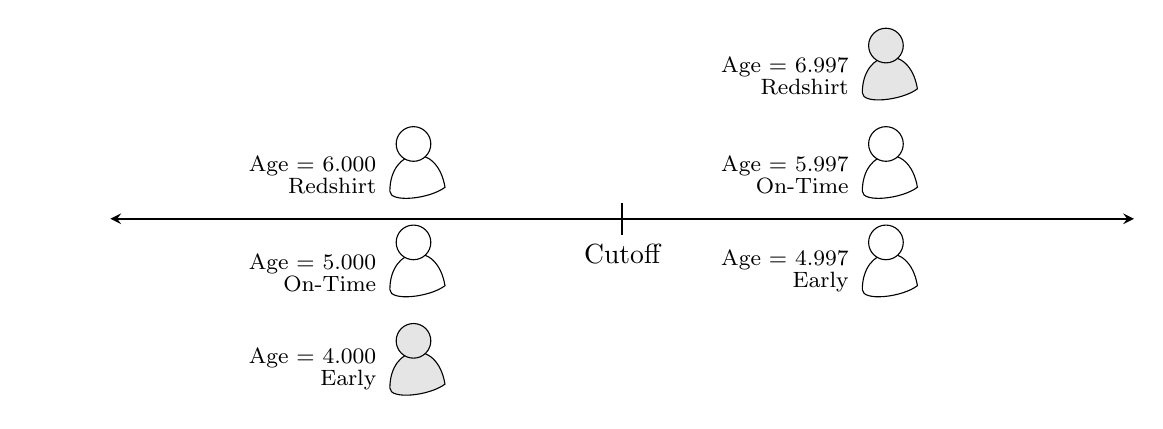
\begin{tikzpicture}

    \draw (-3,-2.25) pic{student={white,<2->}};
    \node (X1) at (-3,-2.25)  [font=\fontsize{8pt}{8pt}\selectfont,anchor=south east,visible on=<2->,align=right] {Age =  5.000 \\ On-Time};
    
    \draw (-3,-1) pic{student={white,<3->}};
    \node (X1) at (-3,-1)  [font=\fontsize{8pt}{8pt}\selectfont,anchor=south east,visible on=<3->,align=right] {Age = 6.000 \\ Redshirt};
    
    \draw (-3,-3.5) pic{student={black!10,<8->}};
    \node (X1) at (-3,-3.5)  [font=\fontsize{8pt}{8pt}\selectfont,anchor=south east,visible on=<8->,align=right] {Age = 4.000 \\ Early};
    
    
    \draw (3,-1) pic{student={white,<5->}};
    \node (X1) at (3,-1)  [font=\fontsize{8pt}{8pt}\selectfont,anchor=south east,visible on=<5->,align=right] {Age = 5.997 \\ On-Time};
    
    \draw (3,-2.25) pic{student={white,<4->}};
    \node (X1) at (3,-2.25)  [font=\fontsize{8pt}{8pt}\selectfont,anchor=south east,visible on=<4->,align=right] {Age = 4.997 \\ Early};
    
    \draw (3,.25) pic{student={black!10,<9->}};
    \node (X1) at (3,.25)  [font=\fontsize{8pt}{8pt}\selectfont,anchor=south east,visible on=<9->,align=right] {Age = 6.997 \\ Redshirt};
    
    
    \draw [font=\fontsize{10pt}{10pt}\selectfont,line width=.1cm,color=white] (-7.5,-1.2) -- (-6.5,-1.2) ;
    \draw [font=\fontsize{10pt}{10pt}\selectfont,line width=.025cm,stealth-stealth,visible on=<3->,] (-6.5,-1.2) -- (6.5,-1.2);
    \draw [font=\fontsize{10pt}{10pt}\selectfont,line width=.025cm,visible on=<3->] (0,-1.4) node [anchor=north] {Cutoff}-- (0,-1.) ;
    \end{tikzpicture}
    
    
    \hyperlink{wait1}{\beamerbutton{Back}}   

\end{frame}



\begin{frame}[label=model1]{\textbf{Modeling kindergarten decisions: first stage}}

\begin{wideitemize}
  \item Given $Z\in \{0,1,2\}$, let the net benefit of treatment be
\begin{align*}
    V_1-V_0 &= \mu_W(Z,X,r) - \nu_W
\end{align*}

\item<2-> If we assume 
\begin{itemize}
    \item Continuity: $F_{\nu}(\cdot|X,r)$, is absolutely continuous
    \item Independence:  $U_W \perp Z|X,r $
    \item Relevance: $\mu_W(Z,X,r)$ is nondegenerate
\end{itemize}

\item<2-> Then $F_{\nu}(\nu_W|X,r):=U_W \sim U[0,1]$ characterizes the first stage:
\begin{align*}
    W &= \mathds{1}(U_W \leq p_z(X,r)) \\
\visible<3>{    p_0 = P(W=1|Z=0,X,r) \hspace{2em} p_1 &= P(W=1|Z=1,X,r) \hspace{4em} p_2 = 1 }
\end{align*}


\end{wideitemize}

\vfill 

\hyperlink{wait1}{\beamerbutton{Back}}   
\end{frame}







\begin{frame}[c,label=educ]{\textbf{These groups are connected to education literature}}

\begin{wideitemize}
\item Wherever $Z$ is as-good-as-random the following hold:
\begin{itemize}
    \item Always takers include redshirters and would-be redshirters with lucky birthdays
    \item Reluctant compliers include early entrants and lucky  would-be early entrants 
    \item Redshirters and early entrants are random samples of always takers and reluctant compliers (respectively)
\end{itemize}

\item My results will estimate effects of waiting on redshirters and early entrants

\item On-Time entrants conflate all groups. The following count as ``on-time entrants'':
\begin{itemize}
    \item Always takers who are assigned to wait (would be redshirters) 
    \item Reluctant compliers who are assigned to start (would be early entrants who start)
    \item Reluctant compliers who are required to wait (would be early entrants who wait)
    \item Eager compliers who are recommended to start
    \item Eager compliers who are recommended or required to wait 
\end{itemize}

\end{wideitemize}

\vfill

\hyperlink{wait1}{\beamerbutton{Back}}   
\end{frame}






\begin{frame}[label=model2]{\textbf{Modeling kindergarten decisions: second stage}}

\begin{wideitemize}
  \item Given unobserved determinants of scores $\gamma_0,\gamma_1$ let potential math scores be
\begin{align*}
    Y(1)=Y_1(X,r,U,\gamma_1) \hspace{3em}&\hspace{3em}    Y(0)=Y_0(X,r,U,\gamma_0)
\end{align*}

\item<2-> If we assume 
\begin{itemize}
    \item Independence:  $(\mu_W,\gamma_0) \perp Z|X,r $ and $(\mu_W,\gamma_1) \perp Z|X,r $
    \item Support: $0<P(W=1|X,r)<1$ % I assume that there are places with P=1...?
    \item Finite Scores: $\mathbb{E}[Y(1)]<\infty$ and $\mathbb{E}[Y(0)]<\infty$
\end{itemize}

\item<2-> Together these imply the LATE monotonicity assumption:
\begin{itemize}
    \item no children would wait if and only if they are recommended to start
    \item no children would start if and only if they are recommended or required to wait
\end{itemize}that


\end{wideitemize}

\vfill 

\hyperlink{wait2}{\beamerbutton{Back}}   
\end{frame}


%------------------------------------------------

\begin{frame}[label=narratives]{\textbf{Common narratives about strategic entry carry implicit assumptions  }}
\begin{wideitemize}

\item Example 1: ``Kindergarten timing is just about readiness''
\begin{itemize}
    \item<2-> Negative selection in levels: $\mu_{0,at}<\mu_{0,ec}<\mu_{0,rc}$ 
    \item<3-> No selection on gains: $\tau_{at}\approx \tau_{ec} \approx \tau_{rc}$ 
\end{itemize}
    
\item<4-> Example 2: ``Surely the privileged kids don't actually gain much''
\begin{itemize}
    \item<5-> Positive selection in levels: $\mu_{0,at}>\mu_{0,ec}>\mu_{0,rc}$ 
    \item<6-> Negative selection on gains: $\tau_{at}<\tau_{ec} < \tau_{rc}$ 
\end{itemize}
% You'll notice this argument is at odds with the equity argument, which requires that AT have a meaningful effect.
    
\item<7-> Example 3: ``Requirements are necessary to ensure readiness''
\begin{itemize}
    \item<8-> No (or positive) selection in levels: $\mu_{0,at}\approx\mu_{0,ec}\approx \mu_{0,rc}$ 
    \item<9-> No stance on selection on gains: $\tau_{at}\lessgtr \tau_{ec} \lessgtr \tau_{rc}$ 
\end{itemize}
      
\item<10-> Estimating these parameters will distinguish between proposed explanations 
% on average
    

\end{wideitemize}

\hyperlink{wait3}{\beamerbutton{Back}}  

\end{frame}




\begin{frame}[label=change]{\textbf{Birthday cutoff policy changes 2002-2022}}
\begin{scaletikzpicturetowidth}{.8\textwidth}
\input{Slides/tables_figures/practice_talk/changes}
        \end{scaletikzpicturetowidth}
\vfill 

\hyperlink{policy1}{\beamerbutton{Back}}   
\end{frame}



%\begin{frame}[label=requirements]{\textbf{Policy details}}

%\begin{wideitemize}
% \item Waiver
 

%\end{wideitemize}

%\vfill 

%\hyperlink{policy1}{\beamerbutton{Back}}   
%\end{frame}




\begin{frame}[label=eclsb,c]{\textbf{Many baseline outcomes are linear in $U_W$}}

\begin{figure}
    \centering
    \includegraphics[width=.8\textwidth]{Draft8/all.pdf}
    
    \footnotesize SOURCE: U.S. Department of Education, National Center for Education Statistics, Early Childhood Longitudinal Survey-Birth Cohort (ECLS-B).
\end{figure}

\hyperlink{redselection}{\beamerbutton{Back}}

\end{frame}



\begin{frame}[label=out,c]{\textbf{Always takers have worse elementary school outcomes}}
\begin{center}
    \resizebox{\textwidth}{!}{
\input{Slides/tables_figures/practice_talk/elementary}}

\end{center}
\hyperlink{redselection}{\beamerbutton{Back}}

\end{frame}




\begin{frame}[label=rdseltest,c]

\frametitle<1-6>{\textbf{Intuition for test of selection}}
\frametitle<7>{\textbf{Intuition: Positive selection}}
\frametitle<8>{\textbf{Intuition: Negative selection}}
\frametitle<9>{\textbf{Data suggest negative selection}}



\begin{center}
\input{Slides/tables_figures/practice_talk/rd_selection}
\end{center}

\hyperlink{redselection}{\beamerbutton{Back}}

\end{frame}















%------------------------------------------------
% Is having AT peers worse than having TC peers
\begin{frame}<0>[label=extensions]{Peer Effects}

Peer effects questions:
    \begin{itemize}
        \item Having older peers improves students' absolute performance \citep{pena2017creating}
        \item Because late entrants are negatively selected and positively affected, this effect might not be the same if a student's older peer is a complier vs always taker...
        \item I've replicated similar results to \citep{pena2017creating}, and preliminary results suggest it is better to have an AT peer than a old complier peer... but I'm not sure I've done it right...
        \item Parental decisions may be socially optimal
    \end{itemize}

\end{frame}



%------------------------------------------------

% LATE sum balance table
\begin{frame}<0>[noframenumbering]{Monotonicity \& Effects Would Resolve Selection Puzzle}

\begin{itemize}
    \item \citet{fortner2017kindergarten} introduce a puzzle of ``negative and postive selection''
    \begin{itemize}
        \item Redshirted students are more likely to have disability diagnosis %lower bound on disability selection
        \item Redshirted students without disabilities perform better on third grade assessments
        \item Redshirted students with disabilities perform worse than peers with disabilities
    \end{itemize}
    \vspace{12pt}
    \item  This characterizes selection in multiple dimensions of covariates
    \vspace{12pt}
    \item Negative selection (i.e., low untreated outcomes) and a large treatment effect could explain both selections but on only one dimension: propensity to be treated
    %\item `Selection on gains' idea: redshirt when it will really help 
    \vspace{12pt}
    \footnotesize
    % Note: this is for students closest to cutoff (63\% of redshirters). Redshirters far from cutoff look to be very negatively selected and I don't estimate the treatment effect for them.
\end{itemize}

\end{frame}

% Parental Preferences 
\begin{frame}<0>{5. Other Ideas}

\citet{cook2018school} show evidence that parents care about relative age less than absolute age. Can I see if they care about relative or absolute performance?
    \begin{itemize}
        \item We could somehow use the changing cutoff date
    \end{itemize}

\vspace{12pt}    
    
Does the difference between AT and TC have something to add about what happens during that year ?
    \begin{itemize}
        \item Both are the same relative and absolute ages
        \item Could the difference say something about what makes up the ``black box'' treatment effect?
    \end{itemize}

\vspace{12pt}
The compulsory schooling laws changed in Michigan near the start of my sample, and while they thought about the cut off, they didn't think as carefully about all four groups
\begin{itemize}
    \item It seems like there is something interesting there beyond the simple policy evaluation
\end{itemize}

\vspace{12pt}

\hyperlink{nextsteps}{\beamerbutton{Back}}

\end{frame}
%------------------------------------------------

%------------------------------------------------
% What is the answer
\begin{frame}<0>{\textbf{Long contributions}}

\only<1>{\vspace{.33em}}
\begin{wideenumerate}
    \item Describe the economics of kindergarten entry using unobserved heterogeneity
    
    \only<1-4>{
    \begin{itemize}
        \item Characterize sorting around recommendations as \textbf<2>{partial compliance}
        % Rather than distinct treatments
        
        {\tiny \color{gray}\citep{black2011too,dhuey2019school,imbens1994identification,angrist1996identification,mogstad2020causal}}
        
        \item Measure selection \textbf<3>{in potential outcomes} between  groups
        % Rather than in covariates
        
        {\tiny \color{gray}\citep{cameron1990effects,graue2000redshirting,march2005academic,schanzenbach2017your,fortner2017kindergarten,cook2018school,fortner2019forced,molnar2018redshirting}}
        
        \item Measure effects \textbf<4>{beyond compliers} from RD-based ``entry age'' analyses
        % Rather than just eager compliers
        
        {\tiny \color{gray}\citep{bedard2006persistence,elder2009kindergarten,elder2010importance,evans2010measuring,black2011too,mccrary2011effect,bedard2012school,cook2016birthdays,kim2017public,black2017simple,bertanha2019external,kowalski2018behavior}}
        
    \end{itemize}}

% Talk about selection and readiness

    
    \item<5-> Quantify the policy tradeoff between recommending vs requiring starting and waiting
    
    \only<5-6>{
    \begin{itemize}
        \item If allowed selection around recommendations  \textbf<6>{increases} achievement but reduce equity
        % Getting the right answer \textbf{depends} on allowing for selection on gains
        
        {\tiny \color{gray}\citep{illinois2019anact}}
        \end{itemize}}
        
    \item<7-> Explore how agents make intergenerational investments under constraints
    \only<7>{
    \begin{itemize}
        
        \item Higher-income families are more responsive to children's gains from waiting, and \hspace{4em} lower-income families are more responsive to the costs of waiting
        
        {\tiny \color{gray}\citep{kline2016evaluating,felfe2018does,cornelissen2018benefits,walters2018demand}}
        % Allowing for het nonparametrically is important
    \end{itemize}}
    
    
    \item<8-> Highlight inequities in how much children benefit from the ``gift of time''
    \only<8>{
    \begin{itemize}
        \item Mechanisms emphasize the role of investments in the year children wait
        
        {\tiny \color{gray}\citep{elder2009kindergarten,shapiro2019if,kline2016evaluating,felfe2018does,cornelissen2018benefits}}
        
        \item Simulations with more prekindergarten for low-SES children raise scores and shrink gaps
        
        %
        
        %If barriers prevent agents from making important investments in their children, it may affect other decisions like school choice, college support, fertility, nutrition, preventative care, and the development of social capital.
        
    \end{itemize}}
\end{wideenumerate}
\end{frame}

\begin{frame}<0>{\textbf{Parental selection increases achievement but reduces equity}}

%\begin{center}
%\input{Slides/tables_figures/practice_talk/intro_results}
%\end{center}
            
\begin{wideitemize}
%\item There is significant selection:
% Recall I am thinking about selection in terms of potential untreated outcomes
\item {\color<1-2>{ptr5}\textbf{Negative selection in levels:}} Parents make lower achieving children wait 
\only<1-2>{
\begin{itemize}
    \item {\color<1-2>{ptb4}\textbf<1-2>{Reluctant waiters}} outperform both other groups when no one waits
    %by more than $0.40\sigma$
    % Talk about readiness
    \item<2-> Selection with {\color<2>{ptr5}\textbf<2>{outcomes}} not characteristics flips common narratives
    
    {\tiny \color{gray}\citep{cameron1990effects,graue2000redshirting,march2005academic,schanzenbach2017your,fortner2017kindergarten}}
    
\end{itemize}}

\item<3-> {\color<3-4>{ptr5}\textbf{Positive selection on gains:}} Strategic entry raises average achievement
\only<3-4>{
\begin{itemize}
    \item {\color<3-4>{ptr5}\textbf{Always waiters'}} gains ($0.60-0.80\sigma$) from waiting are at least double other groups'
    %
    \item<4-> {\color<4>{ptr5}\textbf<4>{Heterogeneity}} beyond the recommendation-LATE matters for policy
    
    {\tiny \color{gray} \citep{bedard2006persistence,elder2009kindergarten,black2011too,mccrary2011effect,bedard2012school,cook2016birthdays}}
\end{itemize}}

\item<5-> {\color<5-6>{ptr5}\textbf{Unequal Impacts:}} Strategic entry expands achievement gaps
\only<5-6>{
\begin{itemize}
    \item Higher-income families benefit 3x more and drive \textit{all} selection on gains
    % to vary by income clarifies that whereas higher-income families select in response to the gains to their children, lower-income families select in response to the costs of waiting.
    \item<6-> Allowing flexible selection may affect other public programs and investments
    
    {\tiny \color{gray} \citep[]{mogstad2018using,kline2019heckits,walters2018demand,sdfas,ito2021selection}}
\end{itemize}}

\item<7-> {\color{ptr5}\textbf<7-9>{Early Investments:}} Public investment could shrink gaps and raise scores

\only<7-9>{
\begin{itemize}
    \item Higher-income families invest more, but similar investments have similar gains
    % to vary by income clarifies that whereas higher-income families select in response to the gains to their children, lower-income families select in response to the costs of waiting.
    \item<8-> Consistent with heterogeneity in take-up and effects of early childhood programs

    {\tiny \color{gray} \citep{kline2016evaluating,felfe2018does,cornelissen2018benefits}}
    
    \item<9-> I compare recommendations, requirements, and expanded public prekindergarten
    
\end{itemize}}

% This is for two reasons...


%\begin{itemize}
%    \item<11-> Average gains are $0.48$ for high SES but only $0.16$ for low SES
%    \item<12-> Only high-income families sort children on gains
%\end{itemize}
\end{wideitemize}



%main implications for what we don't know:
%\begin{itemize}    
%    \item Parents redshirt child if (1) they can AND (2) they think their child needs it
%    \item Parents are making (short term) optimal decisions for their children
%    \item Parents' decisions have (short term) positive externalities for other children
  
\end{frame}


\end{document}



